\section{Свойства вероятности. Некоторые распределения.}
    \subsection{Некоторые дискретные распределения}
        $\mathcal{F} = 2^{\Omega}$, \ $p_1, p_2, \dots \geq 0$, \ $\sum\limits_i^{\infty} p_i = 1$, \ $P(A) := \sum\limits_{i: w_i \in A} p_i$.\\
        Если $|\Omega| = n, \ p_1 = p_2 = \dots = p_n = \frac{1}{n}$ --- получаем классическое определение вероятности.
        \begin{enumerate}
            \item \emph{Биномиальное распределение} $B(n, p)$ ---  распределение количества «успехов» в последовательности из $n$ независимых случайных экспериментов, таких, что вероятность «успеха» в каждом из них постоянна и равна $p$.\\
            $\Omega = \{w = (i_1, \dots, i_n)\}$, $0 < p < 1$ --- фиксированное число.\\
            $P(w) = p^k(1 - p)^{n - k}$\\
            $P(\text{ровно k успехов}) := C_n^kp^k(1 - p)^{n - k}$\\
            $P(\Omega) = \sum\limits_{w}P(w) = \sum\limits_{k = 1}^n C_n^kp^k(1 - p)^{n - k} = (p + 1 - p)^n = 1$
            \item \emph{Геометрическое распределение} --- распределение первого «успеха» в серии испытаний Бернулли ($B(p)$).\\ $\Omega = \{(1), (0, 1), (0, 0, 1), \dots\}$, $0 < p < 1$ --- фиксированное число.\\
            \begin{equation*}
                P(\text{успех наступит на $n$ испытании}) = (1 - p)^{n - 1}p
            \end{equation*}
            \item \emph{Гипергеометрическое распределение} --- в ящике лежат $N$ белых и $M$ черных шаров, вытягивают $n$ шаров.
            \begin{equation*}
                P(\text{вынуто $k$ черных шаров}) = \frac{C_M^kC_N^{n - k}}{C_{M + N}^n}
            \end{equation*}
            \begin{figure}[h!]
				\centering
				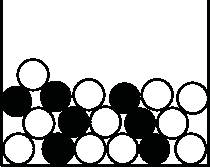
\includegraphics[width=0.3\linewidth]{Lect02/hypergeom.pdf}
				\caption{Гипергеометрическое распределение}
				\label{lect02:pic1}
			\end{figure}
            \item \emph{Пуассоновское распределение} $Pois(\lambda)$ --- число событий, произошедших за фиксированное время, при условии, что данные события происходят с некоторой фиксированной средней интенсивностью ($\lambda$) и независимо друг от друга. $\Omega = \{0, 1, 2, \dots \} \cong \mathbb{N} \cup \{0\}$.\\
            \begin{equation*}
                P\left(\{n\}\right) = \frac{\lambda^ne^{-\lambda}}{n!}
            \end{equation*}
        \end{enumerate}
    \subsection{Геометрические вероятности} 
        $P(A) := \frac{\mu(A)}{\mu(\Omega)}$.
        \begin{enumerate}
            \item \emph{Парадокс Бертрана}. Рассмотрим равносторонний треугольник, вписанный в окружность. Наудачу выбирается хорда окружности. Какова вероятность того, что выбранная хорда длиннее стороны треугольника?
            \begin{enumerate}
                \item \emph{Метод «случайного центра»}. Бросаем точку и проводим через нее хорду, перпендикулярную радиусу. Хорда длиннее стороны равностороннего треугольника, если выбранная точка находится внутри круга, вписанного в треугольник. $P = \frac{\pi{(\frac{R}{2})}^2}{\pi R^2} = \frac{1}{4}$.
                \item \emph{Метод «случайных концов»}. Фиксируем точку на окружности, берем произвольный угол $\alpha$. Чтобы посчитать искомую вероятность, представим, что треугольник повёрнут так, что одна из его вершин совпадает с концом хорды. Заметим, что если другой конец хорды лежит на дуге между двумя другими вершинами треугольника, то длина хорды больше стороны треугольника. Длина рассмотренной дуги равна трети длины окружности, значит, искомая вероятность равна $P = \frac{\frac{1}{3}(2 \pi R)}{2 \pi R} = \frac{1}{3}$.
                \item \emph{Метод «случайного радиуса»}. Случайно выбираем радиус, бросаем на радиус точку и строим через него хорду, перпендикулярную этому радиусу. Хорда длиннее стороны треугольника, если её центр ближе к центру, чем точка пересечения треугольника с зафиксированным радиусом, а сторона треугольника делит радиус пополам. $P = \frac{R}{2R} = \frac{1}{2}$.
            \end{enumerate}
            \begin{figure}[h!]
				\centering
				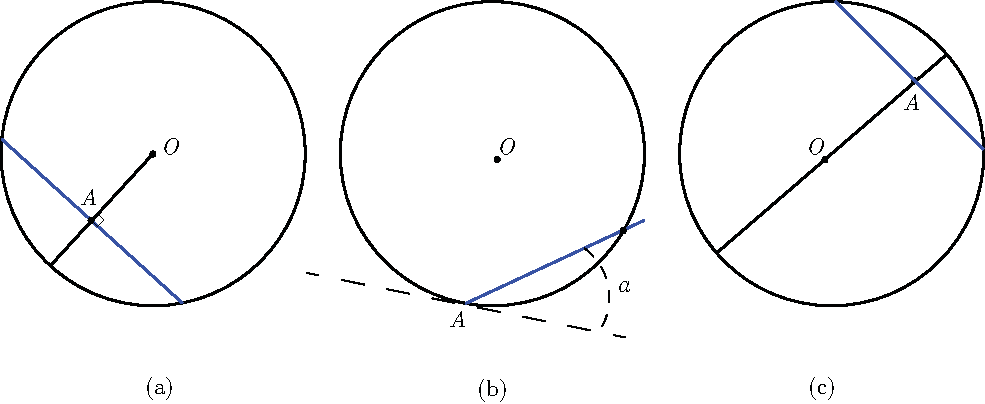
\includegraphics[width=0.6\linewidth]{Lect02/bertrand.pdf}
				\caption{Парадокс Бертрана. Синим отмечена полученная хорда}
				\label{lect02:pic2}
			\end{figure}
            Суть парадокса: проблема точной формализации эксперимента. Тогда и только тогда, когда метод случайного выбора задан, проблема имеет чётко определённое решение.
            \item \emph{Игла Бюффона}. Рассмотрим лист бумаги, расчерченный параллельными прямыми на $n$ полос длины $L$ и ширины $d$ ($|\Omega| = nd \cdot L$). Случайно бросаем на него иглу длиной $l < d$ (случайно выбираем центр $(x, y)$, затем случайно выбираем угол поворота $\alpha$). Какова вероятность того, что игла пересечет одну из линий решетки?\\
            Пусть центр $(x, y)$ оказался в полосе между $(k - 1)$-ой и $k$-ой линией, причем $y > (k - 1)d + \frac{d}{2}$ (случай, где центр находится ближе к $(k - 1)$-ой линии, симметричен). Тогда условие того, что игла, повернутая на угол $0 < \alpha < \pi$ пересекла $k$-ую линию:
            \begin{equation*}
                \begin{cases}
                    kd - \frac{d}{2} < y \leq kd\\
                    kd - y < \frac{l}{2}\sin\alpha
                \end{cases} \implies kd - \frac{l}{2}\sin\alpha < y \leq kd
            \end{equation*}
            Получаем $\int\limits_0^{\pi} (kd - (kd - \frac{l}{2}\sin\alpha))d\alpha = l$ --- для половины полосы.\\
            Искомая вероятность $\P = \frac{2l \cdot nL}{\pi d \cdot nL} = \frac{2l}{\pi d}$.
            \begin{figure}[h!]
				\centering
				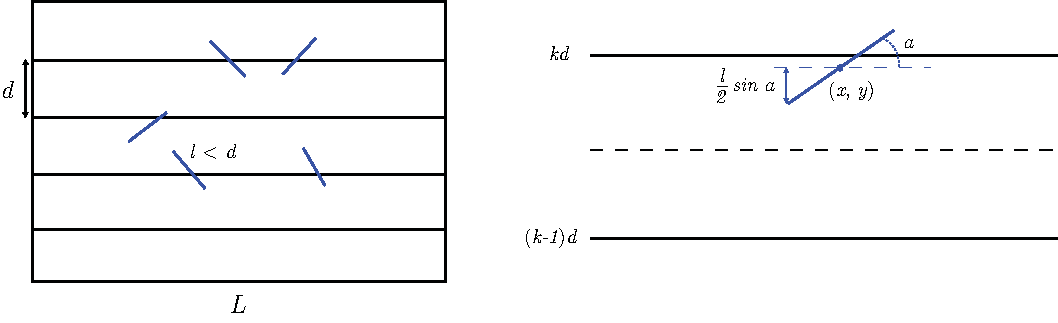
\includegraphics[width=0.9\linewidth]{Lect02/buffon.pdf}
				\caption{Игла Бюффона}
				\label{lect02:pic3}
			\end{figure}
        \end{enumerate}
    \subsection{Свойства вероятностной меры}
        \begin{theorem}\label{lect02:th1}
            Пусть $A, B \in \mathcal{F}$, \ $A_n \in \mathcal{F}$. Справедливы следующие утверждения:
            \begin{enumerate}
                \item $A \subseteq B \implies \P(B \setminus A) = \P(B) - \P(A)$, в частности, $\P(B) \geq \P(A)$
                \item $\P(A \cup B) = \P(A) + \P(B) - \P(AB)$
                \item \emph{(суббадитивность)} $\P(\bigcup\limits_n A_n) \leq \sum\limits_n \P(A_n)$
            \end{enumerate}
        \end{theorem}
        \begin{proof}
            \begin{enumerate}
                \item $B = A \sqcup (B \setminus A) = A \sqcup (B\overline{A})$. Т.к. $A(B \setminus A) = \varnothing$, то $\P(B) = \P(A) + \P(B \setminus A)$.
                \item \begin{equation*}
                    \begin{cases}
                        \P(A \cup B) = \P(A) + \P(B \setminus A)\\
                        \P(B) = \P(AB) + \P(B \setminus A)
                    \end{cases} \implies \P(A \cup B) = \P(A) + \P(B) - \P(AB)
                \end{equation*}
                \item $B_1 = A_1, \ B_2 = A_2 \setminus A_1, \ B_3 = A_3 \setminus (A_1 \cup A_2), \dots$\\
                $\bigsqcup\limits_i B_i = \bigcup\limits_i A_i \implies \P(\bigcup\limits_i A_i) = \P(\bigsqcup\limits_i B_i) = \sum\limits_i \P(B_i) \leq \sum\limits_i \P(A_i)$ (мажорируем ряд).
            \end{enumerate}
        \end{proof}
        \begin{theorem}\label{lect02:th2}
            Пусть $A_1, \dots, A_n \in \mathcal{F}$. Тогда $\P(\bigcup\limits_{i = 1}^n A_i) = \sum\limits_i \P(A_i) - \sum\limits_{i, j} \P(A_iA_j) + \sum\limits_{i, j, k} \P(A_iA_jA_k) - \dots + (-1)^{n - 1}\P(A_1\dots A_n)$.
        \end{theorem}
        \begin{proof}
            По индукции.
        \end{proof}
        \begin{definition}\label{lect02:def1}
             Неотрицательная функция $\mu: \mathcal{A} \implies \mathbb{R}$, $\mathcal{A} \subseteq 2^S$ --- алгебра, называется \emph{счетно-аддитивной}, если $\forall A_1, A_2, \dots \mathcal{A}: A_i \cap A_j = \varnothing \iff i \neq j$ и $\bigcup\limits_i A_i \in \mathcal{A}$ верно равенство $\mu(\bigcup\limits_i A_i) = \sum\limits_i \mu(A_i)$.
        \end{definition}
        \begin{definition}\label{lect02:def2}
             Неотрицательная функция $\mu: \mathcal{A} \implies \mathbb{R}$, $\mathcal{A} \subseteq 2^S$ --- алгебра, называется \emph{непрерывной в нуле}, если $\forall A_n \downarrow \varnothing$ при $n \implies \infty \implies \mu(A_n) \implies 0$ при $n \implies \infty$.
        \end{definition}
        \begin{lemma}\label{lect02:lemma1}
            Пусть $\mu$ --- неотрицательная конечно-аддитивная функция на $\mathcal{A}$ и $\forall A \in \mathcal{A} \ \mu(A) < \infty$. Тогда $\mu \in C(\varnothing) \implies \mu$ непрерывна на монотонных последовательностях: $A_n \downarrow (\uparrow) A$ при $n \implies \infty \implies \mu(A_n) \implies \mu(A)$ при $n \implies \infty$.
        \end{lemma}
        \begin{proof}
            $\forall A \in \mathcal{A} \ \mu(A) < \infty \iff \mu(S) < \infty$. Пусть $A_n \downarrow A \in \mathcal{A}$. Тогда $\mu(A_n \setminus A) \implies 0$ ($\mu$ непрерывна в нуле), а $\mu(A_n \setminus A) = \mu(A_n) - \mu(A) \implies \mu(A_n) \implies \mu(A)$.\\
            Для монотонно возрастающих последовательностей: положим $B_n = \overline{A_n}, B = \overline{A}$. Тогда $B_n \downarrow B \implies \mu(B_n) \implies \mu(B) \implies \mu(S) - \mu(A_n) \implies \mu(S) - \mu(A) \implies \mu(A_n) \implies \mu(A)$ при $n \implies \infty$.
        \end{proof}
        \begin{theorem}\label{lect02:th3}
            Пусть $\mu$ --- конечная неотрицательная функция, заданная на алгебре $\mathcal{A}$ подмножеств $S$. Тогда $\mu$ счетно-аддитивна тогда и только тогда, когда $\mu$ конечно-аддитивна и непрерывна в нуле.
        \end{theorem}
        \begin{proof}
            $\implies$. Пусть $\mu$ счетно-аддитивна, тогда она, очевидно, является конечно-аддитивной. Покажем ее непрерывность в нуле: $A_n \in \mathcal{A} \downarrow \varnothing$. Положим $B_n = A_n \setminus A_{n + 1}$. Очевидно, что $B_iB_j = \varnothing$ при $i \neq j$. Заметим, что $A_n = \bigcup\limits_{k = n}^{\infty}B_k$. $A_1 = \bigcup\limits_{k = 1}^{\infty}B_k \implies \mu(A_1) = \sum\limits_{k = 1}^{\infty} \mu(B_k)$ в силу счетной аддитивности $\mu$. Поскольку ряд сходится, $\mu(A_n) \implies 0$ при $n \implies \infty$.\\
            $\impliedby$. Возьмем $C_k \in \mathcal{A} : C_iC_j = \varnothing$ при $i \neq j$, $\bigcup\limits_k C_k \in \mathcal{A}$. Положим $A_n = \bigcup\limits_{k = n}^{\infty} C_k$. Очевидно, что $A_1 = C_1 \cup C_2 \cup \dots \cup C_{n - 1} \cup A_n$, $n \geq 2 \implies A_n = A_1 \setminus (C_1 \cup \dots \cup C_{n - 1}) \in \mathcal{A}$, причем $C_1, \dots C_{n - 1}, A_n$ попарно не пересекаются.\\
            Очевидно, что $A_n \downarrow \varnothing$ и из конечной аддитивности $\mu(A_1) = \mu(C_1) + \dots + \mu(C_{n - 1} + \mu(A_n))$. Из непрерывности в нуле: $\mu(A_n) \implies 0 \implies \sum\limits_{k = 1}^n \mu(C_k) \implies \mu(A_1) = \mu(\bigcup\limits_{k = 1}^{\infty} C_k) \implies \sum\limits_{k = 1}^n \mu(C_k) = \mu(\bigcup\limits_{k = 1}^{\infty} C_k)$. 
        \end{proof}
        \begin{theorem}\label{lect02:th4}
            Пусть $P, Q$ --- вероятностные меры, заданные на измеримом пространстве $(S, \mathcal{B})$, совпадающие на $\pi$-системе $\mathcal{M}$. Тогда они совпадают на $\sigma (\mathcal{M})$. 
        \end{theorem}
        \begin{proof}
            Положим $\mathcal{D} = \{ A \in \mathcal{B}: P(A) = Q(A)\}$. Тогда по условию теоремы $\mathcal{M} \subseteq \mathcal{D}$. Заметим, что
            \begin{enumerate}
                \item $S \in \mathcal{D}$, т.к. $P(S) = Q(S) = 1$.
                \item $A, B \in \mathcal{D}, \ A \subseteq B \implies B \setminus A \in \mathcal{D}$, т.к. $P(B \setminus A) = P(B) - P(A) = Q(B) - Q(A) = Q(B \setminus A)$.
                \item $A_n \in \mathcal{D}$, $A_n \uparrow A \implies A \in \mathcal{D}$, т.к. $0 = \lim\limits_{n \implies \infty} 0 = \lim\limits_{n \implies \infty} P(A_n) - Q(A_n) = P(A) - Q(A) \implies P(A) = Q(A) \implies A \in \mathcal{D}$ (из непрерывности вероятности).
            \end{enumerate}
            Значит, $\mathcal{D}$ является $\lambda$-системой. По теореме \ref{lect01:th2} $\mathcal{D} = \sigma (\mathcal{M})$.
        \end{proof}
        \begin{theorem}\label{lect02:th5}
            \emph{(Каратеодори)}. Любая вероятностная мера на алгебре $\mathcal{A} \subseteq 2^S$ однозначно продлевается на $\sigma (\mathcal{A})$.
        \end{theorem}
        \begin{proof}
            (схема)
            \begin{enumerate}
                \item Определим внешнюю меру следующим образом: $P^* (A) = \inf \{ \sum\limits_n \P(A_n): A_n \in \mathcal{A}, A \subseteq \bigcup\limits_n A_n \}$. 
                \item Из теоремы \ref{lect02:th1} следует, что можно обойтись покрытиями, состоящими из попарно непересекающихся множеств $A_n \in \mathcal{A}$.
                \item \emph{Оказывается}, что $P^*|_{\mathcal{A}} \equiv P$.
                \item $\forall A, B \in 2^S \ \rho (A, B) = P^*(A \bigtriangleup B)$.
                \item Положим $\mathcal{A}^* = \{ A \in 2^S: \exists A_n \in \mathcal{A} \rho (A_n, A) \implies 0 \text{ при } n \implies \infty \}$. \emph{Очевидно}, что $\mathcal{A} \subseteq \mathcal{A}^*$. 
                \item \emph{Проверяется}, что $\mathcal{A}^*$ --- $\sigma$-алгебра.
                \item \emph{Доказывается}, что $(S, \mathcal{A}^*, P^*)$ --- вероятностное пространство.
            \end{enumerate}
            Единственность продления следует из теоремы \ref{lect02:th4}, т.к. алгебра есть $\pi$-система.
        \end{proof}